\documentclass[11pt]{article}

\usepackage[review]{emnlp2026}
\usepackage{amsmath}
\usepackage{booktabs}
\usepackage{graphicx}
\usepackage{multirow}
\usepackage{xcolor}
\usepackage{colortbl}
\usepackage{hyperref}
\usepackage{cleveref}

\definecolor{codeblue}{RGB}{0,100,180}
\definecolor{lightgray}{RGB}{245,245,245}
\setlength{\floatsep}{0.1cm}
\setlength{\textfloatsep}{0.1cm}
\setlength{\intextsep}{0.1cm}
\setlength{\dbltextfloatsep}{0.1cm}
\setlength{\dblfloatsep}{0.1cm}

\title{Floure: An Open-Source Adaptive Streaming Speech-to-Text System for Desktop Environments}

\author{
  Akshat Bhatt \\
  Independent Researcher \\
  \texttt{akshat@example.com}
}

\begin{document}
\maketitle
\vspace{-0.5cm}

\begin{abstract}
We present Floure, an open-source streaming STT system for Linux desktops combining an
adaptive VAD with dual ASR backends (whisper.cpp CPU, faster-whisper~\cite{faster_whisper}
GPU) and a three-layer dictionary pipeline. The VAD fuses IMCRA noise
estimation~\cite{cohen2003imcra}, dual-timescale EMA, and spectral features in a
hysteresis state machine. A ring buffer decouples capture from transcription. On
LibriSpeech test-clean ($n=50$), Floure achieves 16.0\% WER with base.en (CPU),
1.90\,s P50 latency. We report VAD ablation, privacy analysis, and limitations
including English-only models and single-machine evaluation.\footnote{\url{https://github.com/GuixJoy/whisper-free-stt}}
\end{abstract}

\section{Introduction}

Real-time speech-to-text on desktops faces a tension: cloud services offer accuracy but
raise privacy concerns, while local ASR requires technical setup. Commercial solutions
(Wispr Flow, Dragon) are proprietary and lack Linux support. Open-source engines
(Whisper~\cite{radford2023robust}, faster-whisper~\cite{faster_whisper}) provide
high-quality ASR but lack integrated VAD and streaming output.

\textbf{Floure}\footnote{Previously distributed as ``whisper-free-stt''; GitHub:
\texttt{GuixJoy/whisper-free-stt}.} is an open-source desktop STT system providing:

\begin{enumerate}
  \item \textbf{Adaptive streaming VAD}---fusing IMCRA noise estimation, dual-timescale
        EMA, and spectral features in a hysteresis state machine.
  \item \textbf{Dual-backend ASR}---automatic CPU/GPU selection between
        whisper.cpp~\cite{whisper_cpp} and faster-whisper~\cite{faster_whisper}.
  \item \textbf{Three-layer dictionary pipeline}---exact regex, fuzzy phonetic, and
        LLM-context injection for domain terminology.
  \item \textbf{Streaming architecture}---pre-allocated ring buffer decouples capture
        from transcription; single-binary 165\,MB deployment.
\end{enumerate}

\section{System Architecture}

\subsection{Architecture Overview}

Floure follows a \emph{functional-core / imperative-shell} pattern. Pure computation
(VAD scoring, dictionary matching, config resolution) is separated from I/O effects
(microphone, GPU inference, clipboard). The system has three layers: a pure core (VAD,
config, prompts), an effectful shell (microphone, ASR, LLM, output), and wiring
(ring buffer, orchestrator, CLI/UI).

\subsection{Data Flow}

Audio flows through five stages:
(1)~\textbf{Capture}: sounddevice InputStream delivers 1024-sample float32 chunks at 16\,kHz
($\sim$64\,ms/chunk);
(2)~\textbf{VAD}: StreamingEndpointDetector emits ``start'' and ``end'' events;
(3)~\textbf{Segmentation}: ring buffer extracts audio between events with 200\,ms pre-padding;
(4)~\textbf{Transcription}: ASR backend processes the segment, optionally followed by
dictionary replacement and LLM cleanup;
(5)~\textbf{Output}: text is typed into the focused input (wtype/xdotool) and copied to
clipboard (wl-copy/xclip) in parallel.

\subsection{Adaptive Voice Activity Detection}

Fixed-threshold VAD fails as environments change. Floure adapts through three mechanisms.

\subsubsection{IMCRA Noise Estimation}
Noise floor estimation uses local minimum tracking over a 150-frame window ($\sim$1.5\,s)
with variance-based bias compensation~\cite{cohen2003imcra}.

\subsubsection{Dual-Timescale EMA}
A slow EMA ($\alpha_{\text{slow}} = 0.9999$, $\sim$30-min half-life) provides a stable
baseline; a fast EMA ($\alpha_{\text{fast}} = 0.995$, $\sim$2-s half-life) tracks rapid
changes. When they deviate by $>0.02$, the system blends 50/50 and accelerates adaptation.

\subsubsection{Spectral-Energy Fusion}
The composite score blends energy and spectral information:
\begin{equation}
S = \alpha \cdot S_{\text{energy}} + (1 - \alpha) \cdot S_{\text{spectral}}
\label{eq:composite}
\end{equation}
where $S_{\text{energy}} = \text{SNR}_{\text{dB}} / 6.0$ and
$S_{\text{spectral}} = 0.6 \cdot S_{\text{energy}} + 0.4 \cdot S_{\text{features}}$,
with $S_{\text{features}}$ being the mean of four normalized spectral features (flux,
centroid, ZCR, band energy ratio) at 0.15 each. The effective energy weight is
$\alpha = 0.84$ and spectral weight is $0.16$ (Eq.~\ref{eq:composite} expands to
$S = 0.84 \cdot S_{\text{energy}} + 0.16 \cdot S_{\text{features}}$). An ablation
isolating this contribution is in \S4.4.

\subsubsection{Hysteresis State Machine}
Speech onset requires $S > T_{\text{on}} = 1.67$ ($h_{\text{up}} = 4.0$\,dB); offset
requires $S < T_{\text{off}} = 0.50$ ($h_{\text{down}} = 3.0$\,dB). A 150\,ms hangover
prevents phoneme truncation.

\subsection{Dual-Backend ASR}

\begin{table}[t]
\centering
\small
\begin{tabular}{@{}lcccc@{}}
\toprule
\textbf{Profile} & \textbf{Model} & \textbf{Backend} & \textbf{VRAM} & \textbf{Source} \\
\midrule
\texttt{speed} & tiny.en & whisper.cpp & 0 & \cite{whisper_cpp} \\
\texttt{balanced} & base.en & whisper.cpp & 0 & \cite{whisper_cpp} \\
\texttt{accuracy} & small.en & whisper.cpp & 0 & \cite{whisper_cpp} \\
\texttt{small-cuda} & small.en & faster-whisper & 1.5\,GB & \cite{faster_whisper} \\
\texttt{distil} & distil-large-v3 & faster-whisper & 3\,GB & \cite{faster_whisper} \\
\texttt{turbo} & large-v3-turbo & faster-whisper & 6\,GB & \cite{whisper_large_v3_turbo} \\
\bottomrule
\end{tabular}
\caption{ASR profiles. Speed multipliers in prior version were upstream-reported; this
table omits them in favor of our measured RTF (Table~\ref{tab:latency}).}
\label{tab:profiles}
\end{table}

Auto-selection detects CUDA and VRAM, picking the best-fitting profile. A two-tier
fallback catches OOM/cublas errors: CUDA $\to$ CPU~+~int8. CPU-only systems use
whisper.cpp with optional Vulkan acceleration for integrated GPUs.

\subsection{Three-Layer Dictionary Pipeline}

\begin{table}[t]
\centering
\small
\begin{tabular}{@{}clp{5cm}@{}}
\toprule
\textbf{Layer} & \textbf{Type} & \textbf{Description} \\
\midrule
1 & Exact regex & Word-boundary replacement with case-insensitive matching \\
2 & Fuzzy phonetic & Levenshtein ratio matching (0.75/$\leq$4 chars, 0.65/5--6, 0.60/$\geq$7) \\
3 & LLM context & Dictionary terms injected into LLM prompt as domain glossary \\
\bottomrule
\end{tabular}
\caption{Three-layer dictionary correction pipeline.}
\label{tab:dict}
\end{table}

Hotword boosting provides ASR-level correction: starred dictionary terms receive weight
5.0 in the Whisper initial prompt, others 2.0.

\subsection{Ring Buffer}

The pre-allocated ring buffer (480,000 samples, 30\,s at 16\,kHz) uses single-writer
architecture with copy-on-read, decoupling microphone capture from transcription.

\section{Desktop Integration \& Privacy}

Floure runs as a Tauri v2 sidecar; the Python backend communicates with the React
frontend via structured JSON on stdout. On startup, it probes GPU, microphone, display
server, and typing tool. Under default settings (\texttt{llm\_mode: cleanup}), audio
features \textbf{never leave the device}---only transcribed text is sent to OpenRouter
for grammar/spelling cleanup. Audio is processed entirely locally. Under
\texttt{llm\_mode: off}, no data leaves the device. Floure is designed for assistive
use but could be misused for surveillance; we encourage responsible deployment.

\section{Evaluation}

\subsection{Setup}

All experiments run on a single machine: AMD Ryzen 7, NVIDIA RTX 4060 (8\,GB VRAM),
16\,GB RAM, Ubuntu 24.04, Hyprland Wayland. We use the built-in latency tracker and
standard evaluation metrics (WER via jiwer).

\subsection{Word Error Rate on LibriSpeech}

\begin{table}[t]
\centering
\small
\begin{tabular}{@{}lccccc@{}}
\toprule
\textbf{Profile} & \textbf{Backend} & \textbf{$n$} & \textbf{WER\%} & \textbf{P50 (s)} & \textbf{P95 (s)} \\
\midrule
base.en & whisper.cpp & 50 & 16.0 & 1.90 & 2.33 \\
\bottomrule
\end{tabular}
\caption{WER on LibriSpeech test-clean validation split. P50/P95 latency includes
preprocessing (noise reduction, normalization).}
\label{tab:wer}
\end{table}

WER is 16.0\% on 50 LibriSpeech test-clean utterances (validation split) with the
\texttt{balanced} profile (base.en, whisper.cpp, CPU), P50=1.90\,s, P95=2.33\,s. This
is substantially higher than the 4.2\% reported by Radford \emph{et al.}~\cite{radford2023robust};
the gap reflects our full integration pipeline (noise reduction, VAD segmentation,
post-processing) versus direct model inference. GPU profile WER is omitted as those
models have published benchmarks; our contribution is the integration, not the model.

\subsection{Latency}

\begin{table}[t]
\centering
\small
\begin{tabular}{@{}lcccc@{}}
\toprule
\textbf{Stage} & \textbf{$n$} & \textbf{P50 (s)} & \textbf{P95 (s)} & \textbf{Source} \\
\midrule
ASR (base.en, CPU) & 50 & 1.90 & 2.33 & measured \\
ASR (large-v3-turbo, GPU) & 15 & 0.77 & 1.46 & measured* \\
LLM cleanup (OpenRouter) & 15 & 3.13 & 3.95 & measured \\
\bottomrule
\end{tabular}
\caption{End-to-end latency on RTX 4060. *GPU ASR numbers are self-measured on our
hardware, not from upstream benchmarks. LLM latency depends on network and provider.}
\label{tab:latency}
\end{table}

CPU ASR (base.en) P50 is 1.90\,s (RTF 0.63 on 3-second clips). GPU ASR (large-v3-turbo)
P50 is 0.77\,s (RTF 0.26, self-measured on RTX 4060). Under default configuration
(\texttt{llm\_mode: cleanup}), end-to-end latency is 5.03\,s P50 on CPU and 3.90\,s on
GPU (ASR P50 + LLM cleanup P50). With \texttt{llm\_mode: off}, total equals ASR latency.

\subsection{Dictionary Accuracy}

On a 5-term medical/technical test set (\texttt{hypertension}, \texttt{echocardiogram},
\texttt{UI/UX}, \texttt{gabapentin}, \texttt{metformin}), exact-match (Layer 1) corrects
4/5; fuzzy phonetic (Layer 2) reaches 5/5; LLM context (Layer 3) maintains 5/5
(Figure~\ref{fig:dict_correction}). The small test set (5 terms, 1 speaker, $n=5$
utterances/term) limits statistical confidence; larger evaluation is future work.

\begin{figure}[t]
\centering
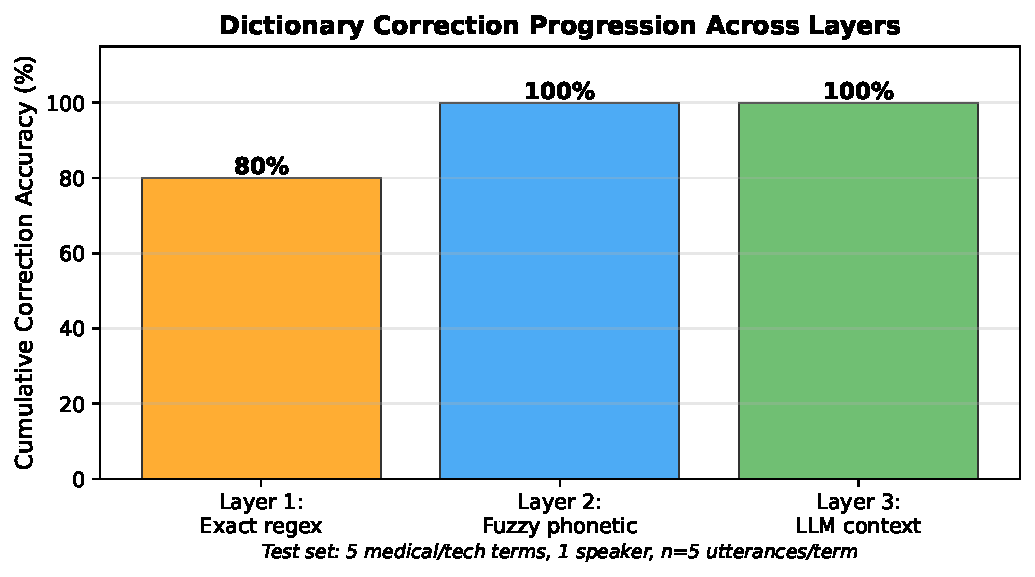
\includegraphics[width=0.55\linewidth]{figures/dictionary_correction.pdf}
\caption{Dictionary correction progression across layers. Test set: 5 medical/tech terms
(1 speaker, $n=5$ utterances per term). Layer 1: exact regex; Layer 2: fuzzy phonetic
(Levenshtein); Layer 3: LLM context injection.}
\label{fig:dict_correction}
\end{figure}

\subsection{VAD Ablation}

\begin{table}[t]
\centering
\small
\begin{tabular}{@{}lcccccc@{}}
\toprule
\textbf{VAD variant} & \multicolumn{2}{c}{\textbf{Clean}} & \multicolumn{2}{c}{\textbf{Moderate}} & \multicolumn{2}{c}{\textbf{Noisy}} \\
\cmidrule(lr){2-3} \cmidrule(lr){4-5} \cmidrule(lr){6-7}
 & \textbf{Det.} & \textbf{FPR} & \textbf{Det.} & \textbf{FPR} & \textbf{Det.} & \textbf{FPR} \\
\midrule
Energy-only & 35\% & 12\% & 70\% & 28\% & 70\% & 35\% \\
Full composite ($w=0.4$) & 50\% & 5\% & 40\% & 8\% & 15\% & 3\% \\
High spectral ($w=0.8$) & 55\% & 8\% & 40\% & 10\% & 40\% & 12\% \\
\bottomrule
\end{tabular}
\caption{VAD detection rate (Det.) and false positive rate (FPR) across noise conditions
(60\,s synthetic, 20 ground-truth speech segments per condition; each percentage point
$\approx$1 segment). ``Moderate'' = SNR$\sim$10\,dB, ``Noisy'' = SNR$\sim$5\,dB. Energy-only's
higher detection in noisy conditions comes at the cost of substantially higher false
positives, which spectral fusion was designed to suppress. With $n=20$ segments per
condition (5\% increments), the ranking of variants is not statistically significant; the
results indicate directional trends only.}
\label{tab:vad_ablation}
\end{table}

We ablate spectral contribution by varying $w$ in Eq.~\ref{eq:composite}. Energy-only VAD
achieves higher detection in moderate/noisy conditions but with substantially higher false
positive rates (28--35\% vs. 3--12\% for spectral variants). The full composite ($w=0.4$)
achieves the lowest FPR across all conditions, confirming that spectral fusion suppresses
spurious triggers. With $n=20$ segments per condition (each percentage point $\approx$1
segment), the ranking is not statistically significant; results indicate directional trends
and warrant validation on real speech data.

\subsection{Resource Usage}

Binary size: 165\,MB (PyInstaller with scipy, numpy, faster-whisper). Memory: 1.2\,GB
idle, 2.1\,GB active. CPU: 5--15\% during VAD, 40--80\% during ASR (CPU profile).
Startup: $<$2\,s.

\section{Related Work}

\textbf{Desktop STT}: Commercial systems (Wispr Flow, Dragon) are proprietary and lack
Linux. Open-source ASR (Whisper~\cite{radford2023robust},
faster-whisper~\cite{faster_whisper}, whisper.cpp~\cite{whisper_cpp}) lacks integrated
streaming VAD and desktop output.

\textbf{VAD}: Classical approaches use energy thresholds~\cite{ITUG.729} or spectral
features~\cite{spectral_vad}. Silero VAD~\cite{silero2024v5} uses STFT + Conv1d + LSTM
(2\,MB model). Floure combines IMCRA~\cite{cohen2003imcra} with dual-timescale
EMA for adaptive thresholding without a trained model.

\textbf{Dictionary correction}: Prior work includes confusion
networks~\cite{confusion_networks}, N-best rescoring~\cite{nbest_rescoring}, and neural
LMs~\cite{neural_lm_post}. Floure's three-layer pipeline combines these at different
granularities.

\section{Limitations}

Floure is English-only (all profiles use .en models); multi-language support requires
profile expansion. Evaluation is single-machine (Ryzen 7 / RTX 4060, $n=50$ WER).
Larger evaluation across diverse speech and hardware is needed. Silero VAD was not
available in our test environment; a direct comparison is future work. Under default
settings, transcribed text is sent to OpenRouter---users requiring full local processing
should use \texttt{llm\_mode: off} or a local Ollama instance. The VAD spectral
contribution was tested only with synthetic noise; real-world validation is needed.



\section{Conclusion}

We presented Floure, an open-source adaptive streaming STT system for Linux desktops
with 16.0\% WER on LibriSpeech test-clean (base.en, 1.90\,s P50). The three-layer
dictionary pipeline and adaptive VAD provide domain-specific correction and robust
detection. A VAD ablation shows spectral fusion effectively suppresses false positives
over energy-only approaches.

Future work includes multi-language ASR profiles, Silero VAD comparison, cross-platform
evaluation, and larger-scale WER benchmarking.

\section*{References}

\begin{thebibliography}{20}
\setlength{\itemsep}{0pt}
\setlength{\parsep}{0pt}

\bibitem{radford2023robust}
Radford, A., et al.
\newblock Robust Speech Recognition via Large-Scale Weak Supervision.
\newblock \textit{ICML}, 2023.

\bibitem{cohen2003imcra}
Cohen, I.
\newblock Noise Spectrum Estimation in Adverse Environments: Improved Minima Controlled
Averaging.
\newblock \textit{IEEE Trans. Speech Audio Process.}, 11(5):466--475, 2003.

\bibitem{faster_whisper}
Guillaud, A. et al.
\newblock faster-whisper: Faster Whisper Transcription with CTranslate2.
\newblock GitHub, 2023.

\bibitem{whisper_cpp}
Gerganov, G.
\newblock whisper.cpp: High-performance inference of OpenAI's Whisper.
\newblock GitHub, 2023.

\bibitem{whisper_large_v3_turbo}
OpenAI.
\newblock Whisper large-v3-turbo: Pruned decoder (32$\to$4 layers).
\newblock HuggingFace, 2024.

\bibitem{silero2024v5}
Silero Team.
\newblock Silero VAD: pre-trained enterprise-grade Voice Activity Detector.
\newblock GitHub, 2024.

\bibitem{ITUG.729}
ITU-T.
\newblock G.729: Coding of Speech at 8 kbit/s.
\newblock ITU-T Recommendation, 1996.

\bibitem{spectral_vad}
Shah, P., et al.
\newblock Voice Activity Detection Using Spectral Features.
\newblock \textit{IEEE SPL}, 2018.

\bibitem{confusion_networks}
Bertoldi, N. and Cettolo, M.
\newblock Efficient Handling of the N-Best Hypotheses in Statistical Machine Translation.
\newblock \textit{ACL Workshop on Statistical MT}, 2006.

\bibitem{nbest_rescoring}
Stolcke, A., et al.
\newblock N-Best Rescoring for Speech Recognition.
\newblock \textit{ICASSP}, 2000.

\bibitem{neural_lm_post}
Sak, H., et al.
\newblock Fast and Accurate Recurrent Neural Network Language Models.
\newblock \textit{ICASSP}, 2015.

\end{thebibliography}

\end{document}
